\documentclass[a4paper,12pt]{article}
\addtolength{\textwidth}{2cm}
\addtolength{\textheight}{2cm}
\addtolength{\footskip}{2cm}
\setlength{\voffset}{-1cm}
\setlength{\hoffset}{-1cm}

\usepackage {graphicx}
\usepackage{natbib}
\usepackage{amssymb,amsmath}
%\usepackage{threeparttable}

\DeclareGraphicsExtensions{.pdf}
\DeclareGraphicsRule{*}{pdf}{*}{}
\graphicspath{{figures/}}
\newcommand{\degree}{$^{\circ}$ }

\title{Pheno Analysis User's Manual\\ Version 1.6}
\author{Reto St{\"o}ckli}

\begin{document}

\maketitle

\begin{center}
\end{center}
\clearpage
\tableofcontents
\clearpage

\begin{abstract}
This is an introduction to the satellite remote sensing data assimilation framework for prognostic phenology models (in short: Pheno Analysis). Pheno Analysis employs sequential ensemble data assimilation by use of the Ensemble Kalman Filter (EnKF) to constrain empirical model parameters and prognostic model states with quality screened Fraction of Photosyntetically Active Radiation absorbed by plants (FPAR) and Leaf Area Index (LAI) observations from NASA's MODIS sensor on board TERRA satellite. The aim of Pheno Analysis is to reduce the uncertainty in globally applicable phenology models in order to make them more realistic for their application within global climate model simulations, especially for those including long term vegetation dynamics and predictions of land surface biogeochemistry coupled to the global carbon and water cycle. The next sections give a short overview for how to set up the Pheno Analysis model and how to run a few exmaples.
\end{abstract}

\section{Introduction}
This document is not a description of the science behind the Pheno Analysis code. Users are strongly motivated to read our two scientific publications \citep{Stockli2008, Stockli2011} and the following publications in order to get familiar with data assimilation \citep{Anderson1999, Anderson2001, Evensen2003, Evensen2004,Ott2004, Moradkhani2005,Aksoy2006}, phenological models \citep{White1997, Chuine2000, Jolly2005} and the land surface datasets from NASA's MODIS sensor \citep{Justice2002, Friedl2002, Hall2002, Hansen2002, Huete2002, Justice2002a, Myneni2002, Schaaf2002, Vermote2002, Wan2002, Cohen2006}. Other datasets used for Pheno Analysis are referenced throughout this document. Users are encouraged to find dataset specifications and uncertainties in those articles.\\

Pheno Analysis has two modes of operation: local-scale and regional-scale. The next sections describe how to exercise two pre-configured examples for both local-scale and regional-scale data assimilation. 

\section{Model description}

\subsection{Local-scale mode}
The local-scale mode is useful to constrain phenological parameters for a single site or for a small area. The current footprint for this mode is set to 0.1\degree longitude x 0.1\degree latitude spacing. The local-scale mode is fully described in \cite{Stockli2008}. The data assimilation evaluates a mixed phenological signal for the chosen site. Phenological parameters will therefore be specific to the chosen site with its vegetation distribution, altitude and climate. Parameters constrained at one site cannot be used to predict phenology at another site.

\subsection{Regional-scale mode}
The regional-scale mode is useful to constrain phenological parameters for large areas or for the earth's entire land surface. The regional-scale mode is documented in a publication \citep{Stockli2011}. The differences to the local-scale mode can be outlined as follows:

\begin{enumerate}
\item the phenology model runs on a grid with 6 dimensions: ensemble members x longitude x latitude x plant functional types x elevation classes x prognostic states. 
\item ECMWF, GEOS 4/5, COSMO or NCEP reanalysis or forecast data are used instead of tower-based meteorology.
\item each MODIS observation is linearly unmixed into a subgrid-scale distribution of 35 plant functional types (pft's) defined by the National Center for Atmospheric Research (NCAR) Community Land Model (CLM) based on a  1 km \% pft distribution map. Update: we have extended the 17 NCAR pft's to 35 pft's by separating the individual crop classes.
\item the ECMWF, NARR, GEOS reanalysis meteorological driver data is downscaled into a subgrid-scale distribution of a user-selectable number of elevation classes based on a 1 km topography map. Simple lapse-rate scaling for temperature is applied, none for radiation and none for humidity.
\item during data assimilation phenological parameters are estimated for each pft separately, or for a selected subset of those pft's. All grid points make use of the same pft-dependent parameters. The parameter matrix $\theta$ has 3 dimensions: ensemble members x pft x model parameters
\item the ensemble matrix $A=(X,\theta)$ is composed of states and parameters. Preliminary findings (unpublished) reveal that the ensemble matrix should be composed of parameters only when simulating larger regions or multiple regions. Parameters are global while states need to be constrained only by a local set of observations. Alternatively, two EnKF filters could be applied: a global one for constraining model parameters and one with a local influence function for constraining prognostic states.
\item data assimilation assigns MODIS observations of FPAR and LAI to predicted FPAR and LAI by use of a model-observation operator where each 1 km MODIS pixel is bilinearly mixed from predicted FPAR and LAI; weighted by \% pft and \% elevation class distribution for this pixel.
\item for output each grid point can be spatially subdivided into subgrid points. The subgrid values are bilinearly mixed from pft and elevation-class dependent FPAR and LAI weighted by subgrid-scale \% pft and elevation distribution.
\item multiple regions can be simultaneously assimilated by use of message passing interface (MPI). For each assimilation step the computing intensive EnKF analysis is performed separately for each region. The updated parameter ensembles for each pft and region are then gathered, and jointly weighted by observation count and variance reduction which results in a single set of phenological parameters which is re-distributed among regions for the next model forecast step.
\end{enumerate}

\section{Directory and File Structure}
In each directory there should be a `README' file containing information of what can be found in the respective directory. The root directory of the Pheno Analysis has the following directory structure:
\begin{verbatim}
bin             : binary files of the compiled Pheno Analysis will be located there
doc             : documentation to the model and datasets
scripts         : wrapper scripts to run the Pheno Analysis
data/ini        : configuration files for example run cases
data/parameters : example phenology prediction parameter sets
data/sites      : geographical domains and names of sites/regions 
src/analysis    : data assimilation and phenology model source code
src/prediction  : stand-alone phenology model prediction code
src/diagnostics : IDL code to analyze the model output
src/utils       : build pft and topography maps, MODIS, ECMWF data
\end{verbatim}

\section{How to compile the model}

\subsection{Unpack the model and the example datasets}
The package can be unpacked by use of the following command:
\begin{verbatim}
tar -zxvf pheno_analysis-VERSION.tar.gz
\end{verbatim}
This will create a folder `pheno\_analysis-VERSION' including all model, script and analysis subdirectories. In the following subsections the root directory is going to be called pheno\_analysis (without the version for simplification). The dataset package can be unpacked by use of the following command:
\begin{verbatim}
tar -zxvf pheno_analysis-datasets.tar.gz
\end{verbatim}
This will create a folder `pheno\_analysis-datasets' including all individual dataset subdirectories needed in the following subsections.

\subsection{Resolve system dependencies}
The following system configuration needs to be present for compiling and running the code:
\begin{itemize}
\item Unix-based operating system 
\item Perl
\item Fortran90/95 and C compiler (currently supported: gcc/gfortran $>=4.4$, pgi $>=9.0$, xlf/xlc, ifort $>=10.0$, pathf90 and Cray programming environment using ftn/cc compiling wrappers)
\item NetCDF library with F90 support ($>=3.6$); compile with the same F90 compiler as the code
\item HDF4 library with F77 support ($>=4.2$, important: disable NetCDF support in the HDF4 library during configure with $--$disable-netcdf, else you run into `multiple symbols' error and warning messages when linking both the NetCDF and HDF4 library) 
\item LAPACK and BLAS or ATLAS if your compiler does not include these math libraries. On OSX, for instance, it is part of the operating system and can be linked to the application by use of the veclib Framework; with PGI Lapack/Atlas are part of the compiler package and should be in the standard PGI compiler library path. For AMD processors, the AMCL could be used for efficiency. For Intel compilers the MKL environment should be used.
\item MPI library, execution and compiler environment (optional)
\item A job submission system like PBS or POE (optional)
\end{itemize}

\subsection{Define the environment}
It makes sense to set your C and Fortran compiler by hand. The configure script will look for one, but may fail to either set the preferred compiler or might choose the C and Fortran compiler from two different programming suites.
\begin{itemize}
\item F90  (executable of Fortran 90 compiler; e.g. `setenv F90 gfortran')
\item CC   (executable of C compiler; e.g. `setenv CC gcc')
\end{itemize}

\subsection{Configure the package}
\begin{verbatim}
cd pheno_analysis/
./configure
\end{verbatim}
You may type:
\begin{verbatim}
./configure --help
\end{verbatim}
in order to find all the configure option. Most likely you will need to add at least the NetCDF and HDF4 library location if they cannot be found in the standard path. For the HDF4 library you will most likely also add the search paths for the JPEG, ZLIB and/or SZIP libraries since the HDF4 library depends finding those dynamically. You will find some shell scripts with the example configure statements for several architectures in the Pheno Analysis root directory:
\begin{verbatim}
config_bluefire.sh    : configuration for the NCAR bluefire Power 6 supercomputer (IBM XL compiler)
config_discover.sh    : configuration for the NASA NCCS discover Linux-cluster supercomputer (Intel Compiler)
config_dole.sh        : configuration for the ETH CSCS Cray XT5 supercomputer (PGI or GCC compiler)
config_narsarsuaq.sh  : configuration for my Macbook Pro (almost a supercomputer) with the GCC compiler installed by fink)
config_rigi.sh        : configuration for the ETH CSCS rigi linux cluster (PGI or GCC compiler)
config_stelia.sh      : configuration for the Colorado State Atmosphere Science Linux cluster (GCC compiler)
\end{verbatim}
If your particular system architecture (e.g. SUN Fortran compiler) is not supported, you will need to add new compiler settings to the configure.ac file, which is then used to generate the Makefile. See the GNU autotools (autoconf and automake) manuals for how to edit the configure.ac file. Please send me a feedback with your updates to configure.ac since other users might want to know these as well.

\subsection{Compile the package}
\begin{verbatim}
make clean
make
make install
\end{verbatim}
This should compile and install the executable 'pheno\_analysis' in the following directory:
\begin{verbatim}
pheno_analysis/bin/
\end{verbatim}
You are advised to currently not make use of the `prefix' statement of the configure command since it will install the executable on a different location disconnected from the rest of the Pheno Analysis framework. This feature might be possible in the future though. If Pheno Analysis does not compile or not link correctly, please check if all required libraries are installed and have Fortran support.

\section{Run the examples}

The Example 1 runs the data assimilation in local-scale mode without pft's at 4 FLUXNET towers \citep{Stockli2008} and the Example 2 runs the data assimilation in regional-scale mode using subgrid-scale 35 pft's and 5 elevation classes \citep{Stockli2011}.

\subsection{Example 1: Local-scale mode}
For the local-scale mode the following datasets are needed:
\begin{itemize} 
\item a map of land cover (MOD12Q1, Collection 4) 
\item the MODIS FPAR/LAI assimilation data (MOD15A2, Collection 5)
\item local-scale tower meteorology
\end{itemize}
The Example 1 datasets for the sites Morgan Monroe State Forest \citep{Schmid2000}, BOREAS NSA Old Black Spruce \citep{Dunn2007}, Tonzi Ranch \citep{Baldocchi2004} and Santarem KM83 \citep{Goulden2004} covering the year 2002 are included in the dataset package `pheno\_analysis\_datasets.tar.gz'. The path to the example datasets and the place where the example should be executed and results are stored however needs to be edited in namelist for the local-scale example. Please therefore edit the following file:
\begin{verbatim}
pheno_analysis/data/ini/analysis_Example1.dat
\end{verbatim}
Find the line where the variable datadir is defined and set it to the location of the unpacked dataset package (no trailing slash /). 
Find the line where the variable rundir is defined and set it to a directory where you want to run your example (the executable, scripts, namelists and output will be written there).
Now run the script:
\begin{verbatim}
cd pheno_analysis/scripts/
./pheno_analysis.pl "Example1"
\end{verbatim}
It will assimilate the 2002 MODIS FPAR/LAI for the 4 tower locations Morgan Monroe State Forest, BOREAS NSA Old Black Spruce, Tonzi Ranch and Santarem KM83 using a 250 ensemble member square-root implementation of Geir Evensen's famous EnKF. The forecast model is integrated on daily time steps and is driven by 30' or 60' tower-based meteorology as predictor data at a single 0.1\degree x 0.1\degree grid point. The one-year assimilation cycle is repeated 5 times, looping over the year 2002. The following initialization and configuration files are used by the above script:
\begin{verbatim}
pheno_analysis/data/sites/sites_example.dat
pheno_analysis/data/ini/analysis_Example1.dat
pheno_analysis/data/ini/forcings_Example1.dat
pheno_analysis/data/ini/observations_Example1.dat
pheno_analysis/data/ini/parameters_Example1.dat
pheno_analysis/data/ini/states_Example1.dat
pheno_analysis/data/parameters/prediction_parameters_local.dat
\end{verbatim}
The following files are created by the above script in the directory rundir/Example1/:
\begin{verbatim}
data/ini/analysis_Example1.dat
data/namelist/domains.dat
data/namelist/phenolist.dat
data/namelist/forcings.dat
data/namelist/observations.dat
data/namelist/parameters.dat
data/namelist/states.dat
data/parameters/prediction_parameters_local.dat
data/sites/sites_example.dat
scripts/pheno_analysis/pl
scripts/read_list.pl
bin/pheno_analysis
\end{verbatim}
The following meteorological driver and boundary data files are used by the Pheno Analysis model:
\begin{verbatim}
pheno_analysis-datasets/MOD12Q1.004/2004001/*.h08v05.*.hdf
pheno_analysis-datasets/MOD12Q1.004/2004001/*.h11v05.*.hdf
pheno_analysis-datasets/MOD12Q1.004/2004001/*.h12v03.*.hdf
pheno_analysis-datasets/MOD12Q1.004/2004001/*.h12v09.*.hdf
pheno_analysis-datasets/MOD15A2.005/2002###/*.h08v05.*.hdf
pheno_analysis-datasets/MOD15A2.005/2002###/*.h11v05.*.hdf
pheno_analysis-datasets/MOD15A2.005/2002###/*.h12v03.*.hdf
pheno_analysis-datasets/MOD15A2.005/2002###/*.h12v09.*.hdf
pheno_analysis-datasets/tower_data/
- BOREAS_NSA_OBS/BOREAS_NSA_OBS_2002.nc
- Morgan_Monroe_State_Forest/Morgan_Monroe_State_Forest_2002.nc
- Santarem_KM83/Santarem_KM83_2002.nc
- Tonzi/Tonzi_2002.nc
\end{verbatim}
The local-scale experiment will run from a minute to a few minutes, depending the speed of your computer. The model's command lline diagnostics should look like this:
\begin{verbatim}
Basedir: /Users/stockli/pheno_analysis Rundir: /Users/stockli/test/Example1 
Creating new runtime environment in: /Users/stockli/test/Example1 
Prediction Parameter file not found : 
/Users/stockli/pheno_analysis/data/parameters/prediction_parameters_local_Example1.dat 
Using Default Parameter file : 
/Users/stockli/pheno_analysis/data/parameters/prediction_parameters_local.dat 
Basedir: /Users/stockli/test/Example1 Rundir: /Users/stockli/test/Example1 
Writing /Users/stockli/test/Example1/data/namelist/domains.dat ...
2002 is not a Leap Year 
Writing /Users/stockli/pheno_analysis/run/test/namelist ...
MPI-support not compiled. Force single process run.


Pheno Analysis Copyright (C) 2010 Reto Stockli (MeteoSwiss)
This program comes with ABSOLUTELY NO WARRANTY
This is free software, and you are welcome to redistribute it
under the terms of the GNU General Public License as published by
the Free Software Foundation, either version 3 of the License, or
any later version. For details see http://www.gnu.org/licenses/gpl.html.


# regions with land area:       1
# processes allocated:          1

Model  grid: nlon,nlat,npft,nhgt:      1     1     1     1
Output grid: nlon,nlat,npft,nhgt:      1     1     1     1
Elevation of single model height level:  259.0 m
mean elevation of model output grid:     259.0 m
No elevation screening of observations applied

Parsing definition file: data/states.dat
Parsing definition file: data/parameters.dat
Parsing definition file: data/force.dat
Parsing definition file: data/observations.dat

Selected Mode: Data Assimilation (analysis):
Process ID:			0
Prediction:			T
Assimilation:			T
Assimilated Parameters:	15
Assimilated States:		4
Ensemble members:		500

...

Total number of parameters updated:         15
Total number of states updated:              4

Day-of-Year :  365
Writing model states/parameters/forcings to file : Tonzi.0000.restart.bin
Writing model parameters to file : Tonzi.parameters_local.dat

Total wall clock      [s]:    60.64
Initialization        [s]:     0.02
Reading Met data      [s]:     0.08
Reading MODIS data    [s]:    22.40
Predicting Phenology  [s]:     0.07
EnKF Solver           [s]:    36.10
MPI synchronizing     [s]:     0.00
Writing output        [s]:     1.95
Successfully exiting model
Phenology Data Assimilation run complete!

\end{verbatim}
The following files are created by the Experiment 1 for the Tonzi Ranch site:
\begin{verbatim}
output/Tonzi.analysis.2002.nc
output/Tonzi.restart.bin
output/Tonzi.parameters_local.2002.1.dat
output/Tonzi.parameters_local.2002.2.dat
output/Tonzi.parameters_local.2002.3.dat
output/Tonzi.parameters_local.2002.4.dat
output/Tonzi.parameters_local.2002.5.dat
log/pheno_global.log
log/pheno_global.err
log/model_successful
\end{verbatim}
A similar file structure is created for the other three sites. The output file is named `Tonzi.analysis.2002.nc'. It is a NetCDF file and only contains the model states of the last loop since it is overwritten for each loop. The file `Tonzi.restart.bin' is a raw binary restart file which is used by Pheno Analysis during yearly restarts, or when a restart is performed at the beginning of the exercise. The resulting parameters files `Tonzi.parameters\_local.2002.[1-5].dat' are plain text files. They contain successively better constrained parameters with each loop (1-5). The .log and .err files are only created when a job submission system is used. The `model\_successful' file is created at the end of each execution of the Pheno Analsys model and tells the wrapper script that the model has been executed until the end of its run loop (not all Fortran compilers allow a return value).

\subsection{Example 2: Regional-scale mode}
The regional-scale mode depends on the following type of datasets:
\begin{itemize} 
\item a map of subgrid-scale pft distribution
\item a map of land surface topography
\item the MODIS FPAR/LAI assimilation data (MOD15A2, Collection 5)
\item meteorological driver data from a gridded reanalysis or forecast dataset
\end{itemize}
Those regional-scale datasets for a sample area around the Colorado Front Range covering the year 2002 are included in the dataset package `pheno\_analysis-datasets.tar.gz'. The path to the example datasets and the place where the example should be executed and results are stored however needs to be edited in namelist for the local-scale example. Please therefore edit the following file:
\begin{verbatim}
pheno_analysis/data/ini/analysis_Example2.dat
\end{verbatim}
Find the line where the variable datadir is defined and set it to the location of the unpacked dataset package (no trailing slash /). 
Find the line where the variable rundir is defined and set it to a directory where you want to run your example (the executable, scripts, namelists and output will be written there).
Now run the script:
\begin{verbatim}
cd pheno_analysis/scripts/
./pheno_analysis.pl "Example2"
\end{verbatim}
This example will assimilate the 2002 MODIS FPAR/LAI for a 0.5\degree x 0.5\degree region around the Colorado Front Range using a 500 ensemble member EnKF. The forecast model integrates on daily steps spanning 25 grid points, 35 pft's and 10 elevation classes. The ECMWF Interim meteorology is used as predictor data, downscaled to 5x5 0.1\degree x 0.1\degree grid points with 5 elevation classes per grid point. The assimilation cycle loops 5 times through 2002 in order to better constrain phenological parameters. The following initialization and configuration files are used by the above script:
\begin{verbatim}
pheno_analysis/data/sites/sites_example.dat
pheno_analysis/data/ini/analysis_Example2.dat
pheno_analysis/data/ini/forcings_Example2.dat
pheno_analysis/data/ini/observations_Example2.dat
pheno_analysis/data/ini/parameters_Example2.dat
pheno_analysis/data/ini/states_Example2.dat
pheno_analysis/data/parameters/prediction_parameters_regional.dat
\end{verbatim}
The following files are created by the above script in the directory rundir/Example2/:
\begin{verbatim}
data/ini/analysis_Example2.dat
data/namelist/domains.dat
data/namelist/phenolist.dat
data/namelist/forcings.dat
data/namelist/observations.dat
data/namelist/parameters.dat
data/namelist/states.dat
data/parameters/prediction_parameters_regional.dat
data/sites/sites_example.dat
scripts/pheno_analysis/pl
scripts/read_list.pl
bin/pheno_analysis
\end{verbatim}
The following meteorological driver and boundary data files are used by the Pheno Analysis model:
\begin{verbatim}
pheno_analysis-datasets/pft/pft.example.nc
pheno_analysis-datasets/topo/topo.example.nc
pheno_analysis-datasets/MOD15A2.005/2002###/*.h09v04.*.hdf
pheno_analysis-datasets/MOD15A2.005/2002###/*.h10v04.*.hdf
pheno_analysis-datasets/ecmwf/interim/*.2002##.nc
\end{verbatim}
The example will take from an hour up to several hours to run, depending on the speed of your computer. This might be a good time to drink coffee, go sleep or have a beer. The parameters are forced to converge slowly in order to account for the sparse temporal information affecting climate control parameters. The model diagnostic output will look like this:
\begin{verbatim}
Basedir: /Users/stockli/pheno_analysis Rundir: /Users/stockli/test/Example2 
Creating new runtime environment in: /Users/stockli/test/Example2 
Prediction Parameter file not found : 
/Users/stockli/pheno_analysis/data/parameters/prediction_parameters_regional_Example2.dat 
Using Default Parameter file : 
/Users/stockli/pheno_analysis/data/parameters/prediction_parameters_regional.dat 
Basedir: /Users/stockli/test/Example2 Rundir: /Users/stockli/test/Example2 
Writing /Users/stockli/test/Example2/data/namelist/domains.dat ...
2002 is not a Leap Year 
Writing /Users/stockli/pheno_analysis/run/test/namelist ...
MPI-support not compiled. Force single process run.


Pheno Analysis Copyright (C) 2010 Reto Stockli (MeteoSwiss)
This program comes with ABSOLUTELY NO WARRANTY
This is free software, and you are welcome to redistribute it
under the terms of the GNU General Public License as published by
the Free Software Foundation, either version 3 of the License, or
any later version. For details see http://www.gnu.org/licenses/gpl.html.


# regions with land area:       1
# processes allocated:          1

Model  grid: nlon,nlat,npft,nhgt:      5     5    35    10
Output grid: nlon,nlat,npft,nhgt:     25    25     1     1
Reading and deriving subgrid-scale topography.
Reading and deriving subgrid-scale pft distribution.

Process ID:      0
Subgrid-scale PFT distribution on output grid: 
PFT    1 type: bar_all   :   14.3 % of area. Selected: T
PFT    2 type: enf_tem   :    9.0 % of area. Selected: T
PFT    3 type: enf_bor   :    6.8 % of area. Selected: T
PFT    4 type: dnf_bor   :    0.0 % of area. Selected: F
PFT    5 type: ebf_tro   :    0.0 % of area. Selected: F
PFT    6 type: ebf_tem   :    0.0 % of area. Selected: F
PFT    7 type: dbf_tro   :    0.0 % of area. Selected: F
PFT    8 type: dbf_tem   :    2.6 % of area. Selected: T
PFT    9 type: dbf_bor   :    1.1 % of area. Selected: F
PFT   10 type: ebs_all   :    0.0 % of area. Selected: F
PFT   11 type: dbs_tem   :    9.2 % of area. Selected: T
PFT   12 type: dbs_bor   :    4.2 % of area. Selected: T
PFT   13 type: c3g_arc   :    1.4 % of area. Selected: F
PFT   14 type: c3g_nar   :   33.5 % of area. Selected: T
PFT   15 type: c4g_all   :    0.1 % of area. Selected: F
PFT   16 type: cro_brl   :    0.7 % of area. Selected: F
PFT   17 type: cro_cas   :    0.0 % of area. Selected: F
PFT   18 type: cro_cot   :    0.0 % of area. Selected: F
PFT   19 type: cro_grn   :    0.0 % of area. Selected: F
PFT   20 type: cro_mze   :    3.6 % of area. Selected: T

...

Starting EnKF Analysis on DoY:  364
Global Analysis Mode for Parameter Estimation
Total Number of valid observations:       1348
Total Number of gridded observations:       50

Total number of parameters updated:        525
Total number of states updated:           8100

Day-of-Year :  365
Writing model states/parameters/forcings to file : Colorado_Front_Range.0000.restart.bin
Writing model parameters to file : Colorado_Front_Range.parameters_regional.dat

Total wall clock      [s]:   418.78
Initialization        [s]:     0.77
Reading Met data      [s]:     2.93
Reading MODIS data    [s]:    21.06
Predicting Phenology  [s]:   163.63
EnKF Solver           [s]:   199.30
MPI synchronizing     [s]:     0.00
Writing output        [s]:    29.50
Successfully exiting model
Phenology Data Assimilation run complete

\end{verbatim}
The following files are created by the regional-scale Pheno Analysis model for the Colorado Front Range area in the directory rundir/Example2/:
\begin{verbatim}
output/Colorado_Front_Range.analysis.2002.nc
output/Colorado_Front_Range.restart.bin
output/Colorado_Front_Range.parameters_regional.2002.1.dat
output/Colorado_Front_Range.parameters_regional.2002.2.dat
output/Colorado_Front_Range.parameters_regional.2002.3.dat
output/Colorado_Front_Range.parameters_regional.2002.4.dat
output/Colorado_Front_Range.parameters_regional.2002.5.dat
log/pheno_global.log
log/pheno_global.err
log/model_successful
\end{verbatim}
The output NetCDF file `Colorado\_Front\_Range.analysis.2002.nc' contains all predicted phenological states  for the final assimilation loop (5). The output grid is subdivided 5x5 times for each model forecast grid point, resulting in 25 x 25 grid points. The subgrid-scale pft's and elevation classes are aggregated for the output (can be changed in the above perl script). The file `Colorado\_Front\_Range.restart.bin' contains raw binary restart used for yearly restarts. `Colorado\_Front\_Range.parameters\_regional.2002.[1-5].dat' contain successively constrained model parameters by pft for each of the assimilation loops (1-5). The .log and .err files are only created when a job submission system is used. The `model\_successful' file is created at the end of each execution of the Pheno Analsys model and tells the wrapper script that the model has been executed until the end of its run loop (not all Fortran compilers allow a return value).

\section{Analyze the Output}

\subsection{Example 1: Local-scale mode}
The following IDL code can be used to analyze local-scale model output:
\begin{verbatim}
src/diagnostics/phenology_local.pro
\end{verbatim}
No documentation is provided for my analysis tools. Comments are written into the IDL code though. The user may use these programs and find some hints on how to start analyzing the model output. The following figures enable to check whether the local-scale example did run successfully or not. Figure~\ref{figure: local 1} and Figure~\ref{figure: local 2} display how during the first year of assimilation model states and parameters start to change by the constraining MODIS observations. States and parameters have a large ensemble spread at the beginning. Structural vegetation parameters and prognostic states become defined well after only a one year long data assimilation for most sites.\\ 

It takes longer to constrain climate control parameters as described in \cite{Stockli2008}. Figure~\ref{figure: local 3} demonstrates that after 5 years of assimilation (we only have a single year of data, but we loop 5 times over that year) the predictive capability of the model has greatly improved. The prognostic model states further do not respond much more to the observations after such a period. There is still some potential to better constrain model parameters with more data or longer time series, especially for sites with few high quality observations like for instance at Santarem KM83.

\begin{figure}[hp]
\begin{center}
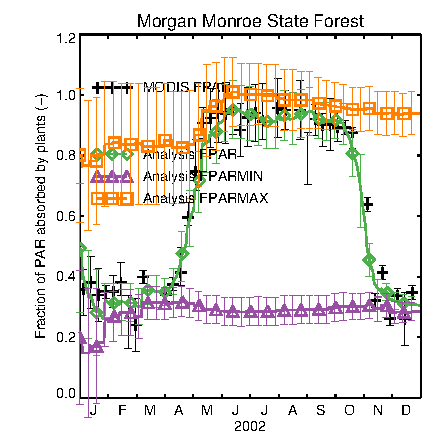
\includegraphics[scale=1.0]{Morgan_Monroe_State_Forest.dayplot.2002.FPAR.MODIS.pdf}
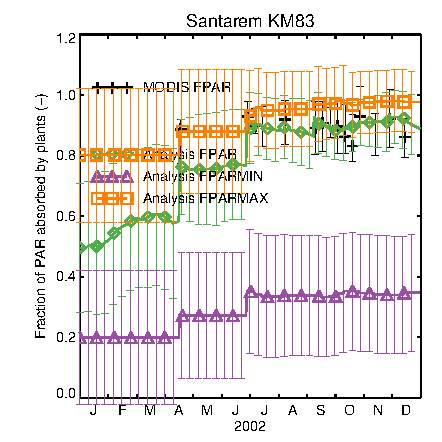
\includegraphics[scale=1.0]{Santarem_KM83.dayplot.2002.FPAR.MODIS.pdf}
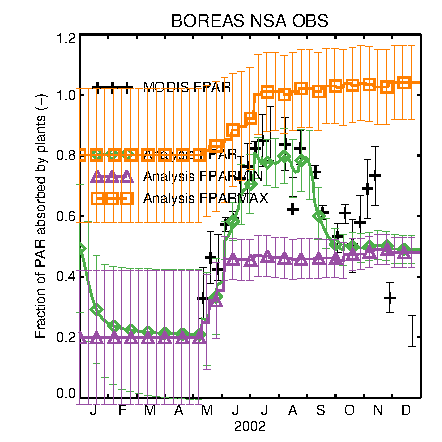
\includegraphics[scale=1.0]{BOREAS_NSA_OBS.dayplot.2002.FPAR.MODIS.pdf}
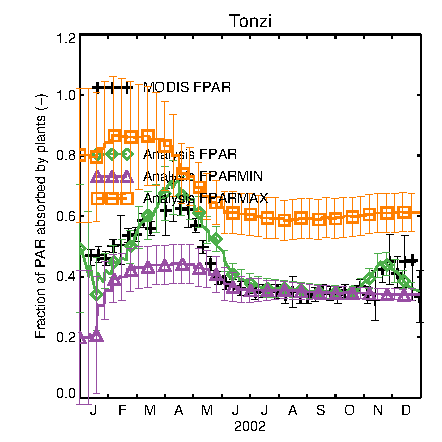
\includegraphics[scale=1.0]{Tonzi.dayplot.2002.FPAR.MODIS.pdf}
\caption{First year (loop=1) of the data assimilation cycle using the local-scale mode: model prognostic state FPAR and the two structural model parameters FPAR$_{max}$ and FPAR$_{min}$ are sequentially constrained by the MODIS FPAR (shown) and LAI (not shown) observations.}
\label{figure: local 1}
\end{center}
\end{figure}

\begin{figure}[hp]
\begin{center}
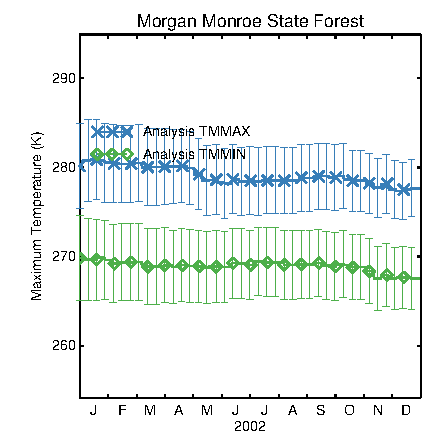
\includegraphics[scale=0.5]{Morgan_Monroe_State_Forest.dayplot.2002.TMMAX.MODIS.pdf}
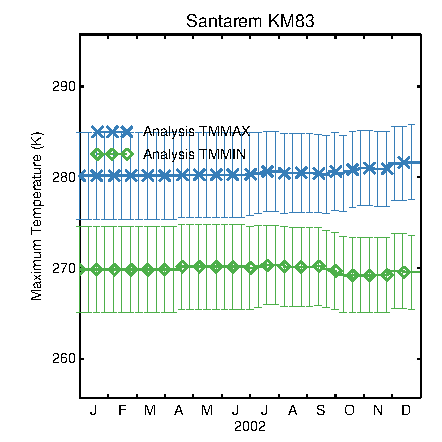
\includegraphics[scale=0.5]{Santarem_KM83.dayplot.2002.TMMAX.MODIS.pdf}
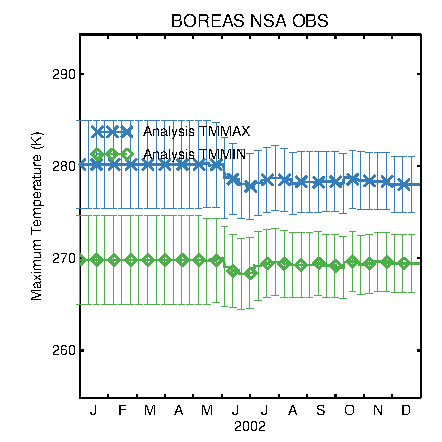
\includegraphics[scale=0.5]{BOREAS_NSA_OBS.dayplot.2002.TMMAX.MODIS.pdf}
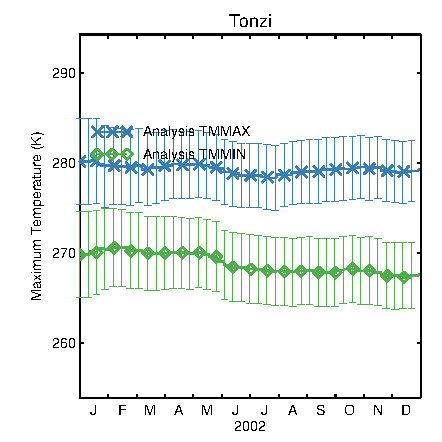
\includegraphics[scale=0.5]{Tonzi.dayplot.2002.TMMAX.MODIS.pdf}
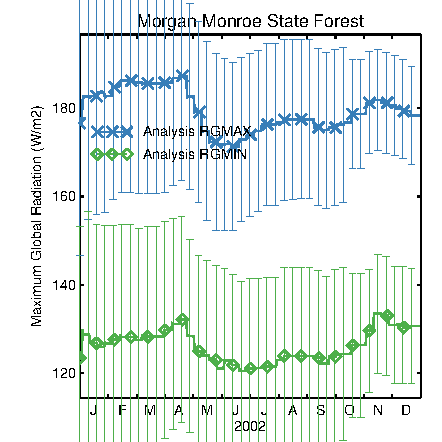
\includegraphics[scale=0.5]{Morgan_Monroe_State_Forest.dayplot.2002.RGMAX.MODIS.pdf}
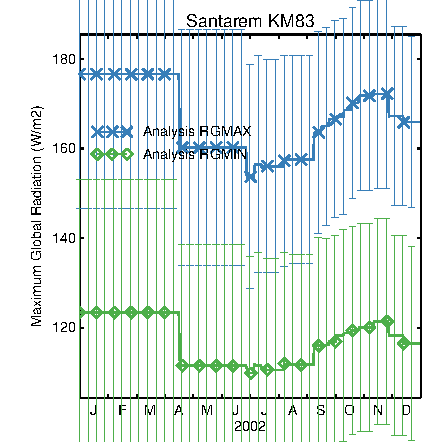
\includegraphics[scale=0.5]{Santarem_KM83.dayplot.2002.RGMAX.MODIS.pdf}
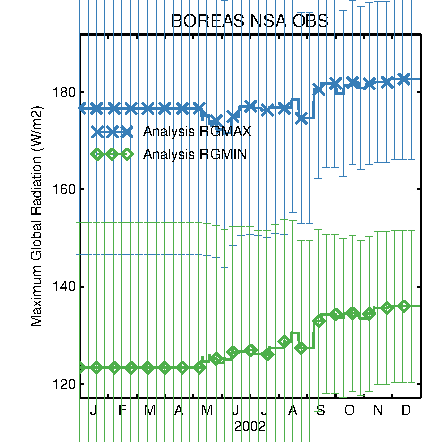
\includegraphics[scale=0.5]{BOREAS_NSA_OBS.dayplot.2002.RGMAX.MODIS.pdf}
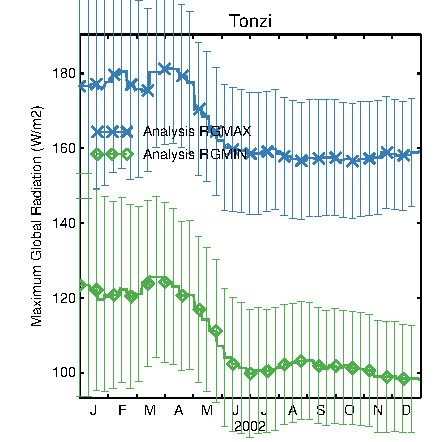
\includegraphics[scale=0.5]{Tonzi.dayplot.2002.RGMAX.MODIS.pdf}
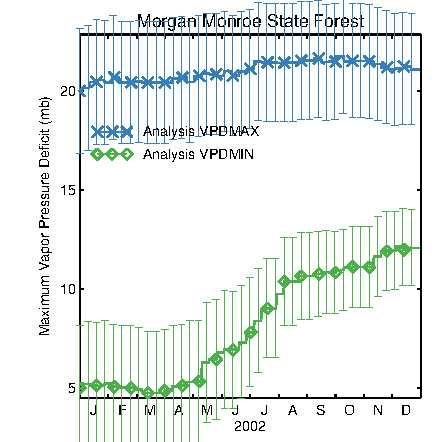
\includegraphics[scale=0.5]{Morgan_Monroe_State_Forest.dayplot.2002.VPDMAX.MODIS.pdf}
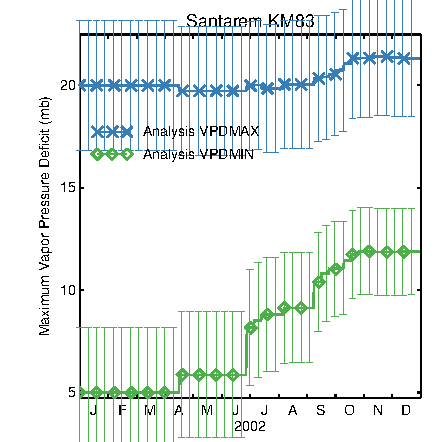
\includegraphics[scale=0.5]{Santarem_KM83.dayplot.2002.VPDMAX.MODIS.pdf}
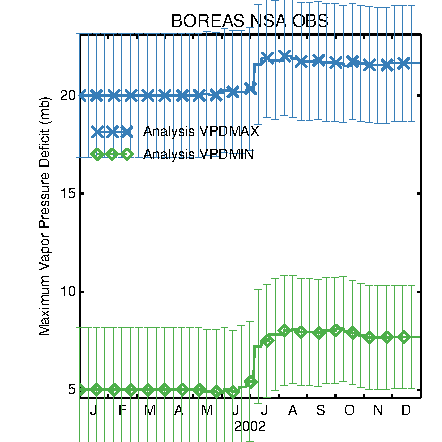
\includegraphics[scale=0.5]{BOREAS_NSA_OBS.dayplot.2002.VPDMAX.MODIS.pdf}
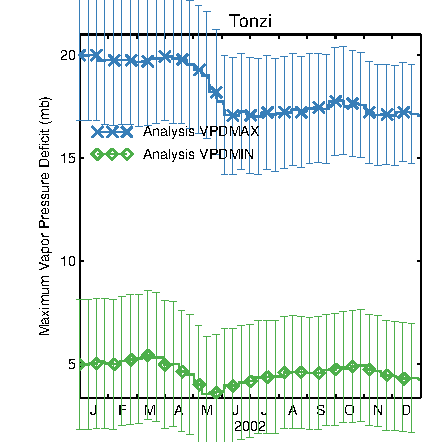
\includegraphics[scale=0.5]{Tonzi.dayplot.2002.VPDMAX.MODIS.pdf}
\caption{First year (loop=1) of the data assimilation cycle using the local-scale mode: model climate parameters are sequentially constrained by the MODIS FPAR (shown) and LAI (not shown) observations. .}
\label{figure: local 2}
\end{center}
\end{figure}

\begin{figure}[hp]
\begin{center}
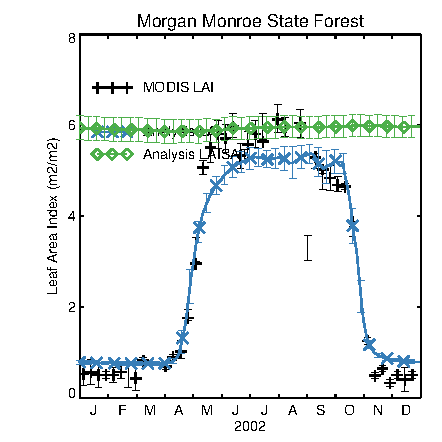
\includegraphics[scale=1.0]{Morgan_Monroe_State_Forest.dayplot.2002.LAI.MODIS.pdf}
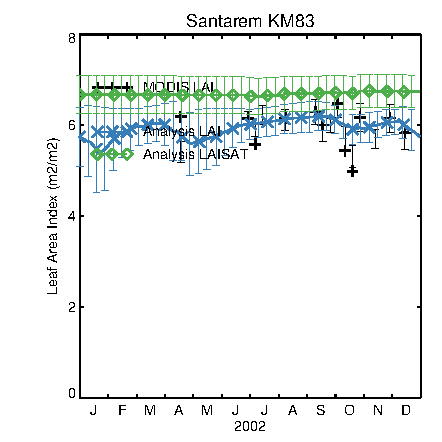
\includegraphics[scale=1.0]{Santarem_KM83.dayplot.2002.LAI.MODIS.pdf}
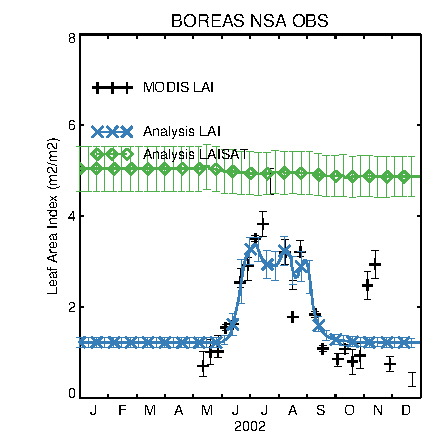
\includegraphics[scale=1.0]{BOREAS_NSA_OBS.dayplot.2002.LAI.MODIS.pdf}
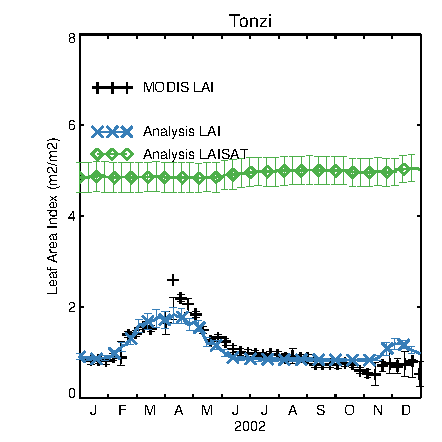
\includegraphics[scale=1.0]{Tonzi.dayplot.2002.LAI.MODIS.pdf}
\caption{Fifth year (loop=5) of the data assimilation cycle using the local-scale mode: model prognostic state LAI and the structural model parameter LAI$_{max}$ are both much better defined after constraining them with 5 years of MODIS FPAR (shown) and LAI (not shown) observations.}
\label{figure: local 3}
\end{center}
\end{figure}

\clearpage

\subsection{Example 2: Regional-scale mode}
The following IDL code can be used to analyze regional-scale model output:
\begin{verbatim}
src/diagnostics/phenology_regional.pro
\end{verbatim}
No documentation is provided for my analysis tools. Comments are written into the IDL code though. The user may use these programs and find some hints on how to start analyzing the model output. The right-hand side of Figure~\ref{figure: regional 1} displays FPAR simulated on the chosen output grid consisting of 25 x 25 grid points. The FPAR value of each output grid point is aggregated from a predicted subgrid-scale distribution of pft- and elevation-dependent FPAR consisting of 35 plant functional types, of 10 elevation classes and of 500 ensemble members. Similar output diagnostics can be derived for LAI and other prognostic model states. The left-hand side of Figure~\ref{figure: regional 1} shows corresponding MODIS-observed and quality screened FPAR on the same output grid. Missing values are common since not all MODIS observations pass the quality check. Observation uncertainty, which plays an important role during data assimilation, is not shown.\\

Interpretation of Figure~\ref{figure: regional 1}: at the beginning of the assimilation cycle all 35 plant functional types have the same phenological model parameters assigned. Therefore all model output grid points look pretty much the same (top panel). During the first year (center panel) parameters begin to slowly  adjust, depending on the number of and on the quality of the satellite observations. After the fifth year of data assimilation (bottom panel) the spatial structure of the modeled phenology becomes closer to the one in the observations because the model has learned from the MODIS data how a certain plant functional type at a specific elevation (and therefore also climate) responds to the driving climatic forcing. 

\begin{figure}[hp]
\begin{center}
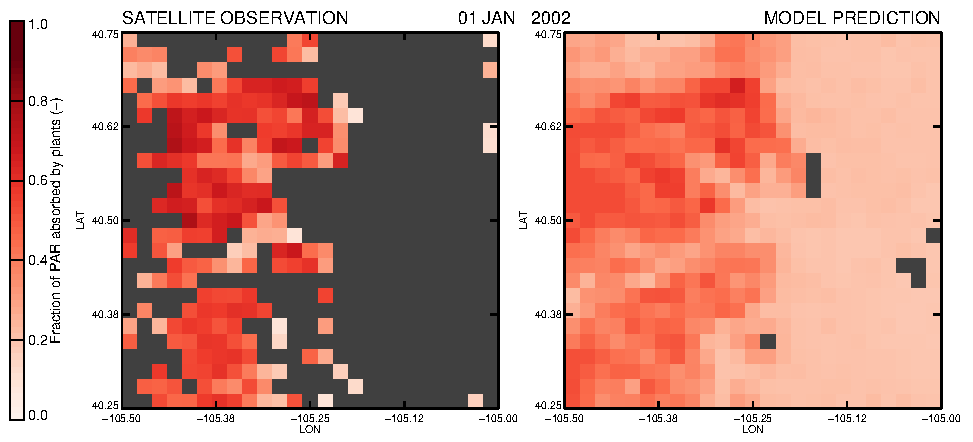
\includegraphics[scale=0.8]{Colorado_Front_Range.FPAR.test.20020101.pdf}
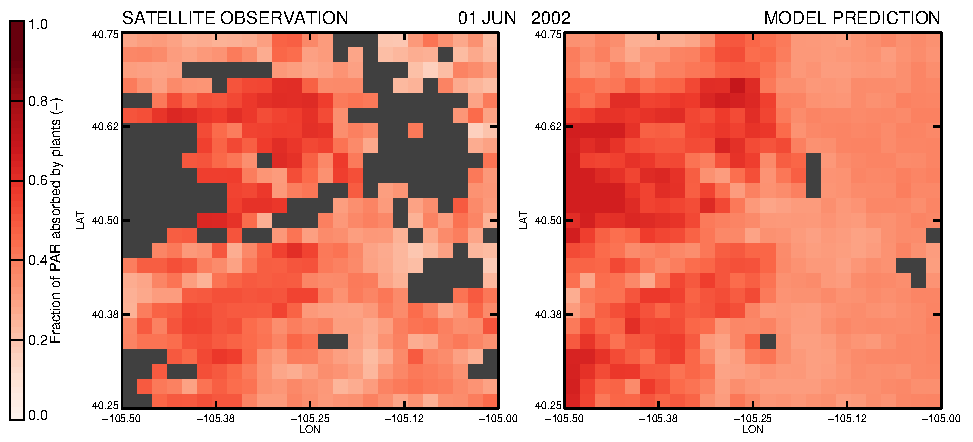
\includegraphics[scale=0.8]{Colorado_Front_Range.FPAR.test.20020601.pdf}
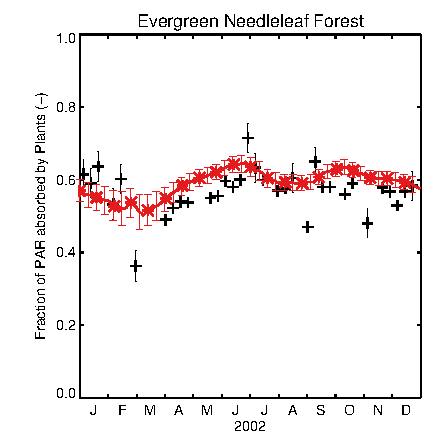
\includegraphics[scale=0.8]{ENF.FPAR.test.2002.pdf}
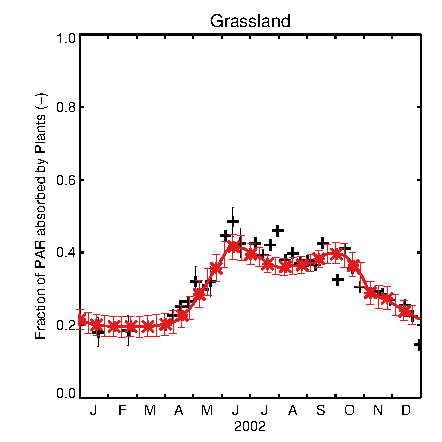
\includegraphics[scale=0.8]{GRA.FPAR.test.2002.pdf}
\caption{Top 4 panels: observed and Predicted FPAR of the regional-scale data assimilation with a 0.5\degree x 0.5\degree area of the Colorado Front Range on 1 January and 1 June. The 2002 MODIS observations were cycled 5 times in order to better constrain parameters. Bottom 2 panels: the pft-dependent phenological parameters for the region have nicely captured the temporal patterns of the Colorado Front Range evergreen needleleaf forest phenology (left) in the Rocky Mountain area to the west and the phenology of the grasslands (right) to the east of the assimilation domain.}
\label{figure: regional 1}
\end{center}
\end{figure}

The success of this regional-scale modeling approach also largely depends on the quality of the underlying \% pft distribution map, the topography map and of the realism of the employed climate downscaling. The parameters for a regional-scale or even global-scale experiment show a much slower convergence and variance reduction than for the local-scale case because there are more degrees of freedom in the ensemble matrix (35 pft's x number of parameters, if no states are assimilated, compared to a single pft x number of parameters in the local-scale case). Due to the higher number of observations on a regional grid (around 5000-10000 observations per \degree longitude x \degree latitude region), observational noise can limit the effectiveness of the the cost function minimization within the EnKF. More ensemble members would be needed, leading to greatly increased computing costs.\\

Based on these preliminary findings in the operation of the regional-scale Pheno Analysis, the following future developments are planned for upcoming model versions:
\begin{itemize}
\item include the Mean Likelyhood Ensemble Filter (MLEF \citep{Zupanski2005, Albayrak2007}) which has a better treatment of the cost function gradient and therefore needs less ensemble members than EnKF.
\item better distribute global EnKF solver among MPI processes. Right now the global EnKF solver is carried out on a single process that collects the global observations, or super-observations.
\item check out MODIS Collection 6 land products
\item use MODIS on AQUA and TERRA data streams
\item create a better pft map with a new MOD44 VCF dataset (Collection 5 of this dataset is not available yet)
\item parallel NetCDF implementation, required a better.
\item include other phenology models (such as the ones presented in \cite{Stockli2008}.
\item generalize the Pheno Analysis framework for other satellite remote sensing parameters such as radiative surface temperature, NDVI, GPP, albedo, solar radiation from geostationary satellites or snow cover. Pheno Analysis could be extend to a full land data assimilation system to constrain a significant number of uncertainties in land surface models (not just the phenology). This is unlike current land data assimilation systems used for state assimilation (such as the NASA's LIS, LDAS, GLDAS). The idea is to make land surface models look and feel the same as observed by the best available remote sensing data and ground measurements through the above model-data fusion process. Assimilating globally applicable model parameters instead model states guarantees that the model's realism is increased for their application in past or future climate simulations where no satellite data can be used to constrain model states.
\end{itemize}

\section{Simulate a phenological hindcast or forecast}
Use the Pheno Analysis framework without the data assimilation option but with constrained parameter sets: put the assimilated parameter set into the pheno\_analysis/data/parameters/ directory with the file name prediction\_parameters\_local\_EXPERIMENTNAME.dat or prediction\_parameters\_regional\_EXPERIMENTNAME.dat and run the Pheno Analysis with the option analysis=0 set in the analysis\_EXPERIMENTNAME.dat namelist file.

\section{Prepare additional datasets}
In order to exercise Pheno Analysis at other locations than the four FLUXNET tower sites or than the Colorado Front Range region, additional datasets not part of the example dataset package have to be downloaded or generated. A global dataset cannot be part of the example dataset due to size limits. All additional datasets (except the ECMWF ERA-40 and Interim reanalysis) are either publicly available, or they can be generated by use of the dataset utilities included with the Pheno Analysis package.

\subsection{Topgraphy data}
The example topography dataset for the Colorado Front Range is located in:
\begin{verbatim}
pheno_analysis-datasets/topo/
\end{verbatim}
The following IDL code can be used to modify or enlarge it:
\begin{verbatim}
src/utils/topo/maketopo.pro
\end{verbatim}
It depends on the International  Centre for Tropical  Agriculture (CIAT) CGIAR Space Shuttle Topography Mission (SRTM) dataset \citep{CGIAR-SRTM} and the United States Geological Survey (USGS) GTOPO30  \citep{GTOPO1996} dataset. Those datasets are not part of the example dataset package (too large for distribution) but they are available for downloaded on public web servers. For instructions visit the README file in the above IDL code directory.

\subsection{Plant functional type data}
The example plant pft dataset for Morgan Monroe State forest is located in:
\begin{verbatim}
pheno_analysis-datasets/pft/
\end{verbatim}
The following IDL code can be used to modify or enlarge it:
\begin{verbatim}
src/utils/pft/makepftclim.pro
\end{verbatim}
It depends on the presence of these datasets:
\begin{enumerate}
\item MOD15A2 Collection 005 MODIS FPAR/LAI dataset 2001-2007 \citep{Myneni2002, Justice2002}
\item MOD12Q1 Collection 004 MODIS land cover dataset, 2004/001 \citep{Friedl2002}
\item MOD44B Collection 003 MODIS Vegetation Continuous Fields dataset \citep{Hansen2005}
\item AVHRR Tree Cover Continuous Fields tree cover and leaf type dataset \citep{Defries2000a}
\item The Leff et al. global crop dataset including 18 crop types \cite{Leff2004}
\item Wilmott and matsuura global 0.5\degree temp + precip dataset \citep{Wilmott2007}
\item topography dataset for selected area, previously created in above subsection
\end{enumerate}
Those datasets are not part of the example dataset package (too large for distribution)  but they are available for downloaded on public web servers. For instructions visit the README file in the above IDL code directory or visit the README files in the respective dataset directories.

\subsection{Land cover data}
Other MOD12Q1 Collection 004 L3 MODIS land cover \citep{Friedl2002} tiles than the four tiles in the example dataset package can be downloaded by following the instructions in the README file found in the directory:
\begin{verbatim}
pheno_analysis_datasets/MOD12Q1.004/
\end{verbatim}

\subsection{MODIS FPAR/LAI assimilation data}
The MOD15A2 Collection 005 MODIS FPAR/LAI dataset \citep{Myneni2002, Justice2002} is the primary observation source for the data assimilation. It is also used to distribute C3 and C4 grassland when creating the pft map (see above). Four sets of tiles for 2002 covering the example regions are located in:
\begin{verbatim}
pheno_analysis-datasets/MOD15A2.005/
\end{verbatim}
Other L3 tiles can be manually downloaded from NASA's WIST interface like the MOD12Q1 tiles. I have created a perl script which allow to automatically fetch all land tiles for a given time period or selected tiles. The script is located in:
\begin{verbatim}
src/utils/modis/
\end{verbatim}

\subsection{ECMWF Interim/ERA-40 reanalysis}

ECMWF ERA-40 \citep{Uppala2005} and Interim (reference?) reanalysis data serves as the predictor data for regional-scale data assimilation experiments. For Morgan Monroe State Forest region a subset for the year 2002 is provided here:
\begin{verbatim}
pheno_analysis-datasets/ecmwf/interim/
\end{verbatim}
Users who would like to have the full global coverage and the 1957-2001 (ERA-40), 1989-2008 (Interim) time series need to get access to the ECMWF MARS archive. The following scripts will then enable to a) extract GRIB fields from ECMWF MARS and b) transform them into monthly NetCDF files:
\begin{verbatim}
src/utils/ecmwf/
\end{verbatim}

\subsection{NCEP NARR reanalysis}
NCEP NARR reanalysis data \citep{Mesinger2006} can be used as the predictor data for regional-mode data assimilation experiments. No NARR data is currently supplied with the example dataset package. The NARR reading and reprojection routine further needs updating and cannot be used as-is.

\subsection{Tower meteorology}
Tower meteorology from the FLUXNET project \citep{Baldocchi2001} for the sites Morgan Monroe State Forest, BOREAS NSA Old Black Spruce, Tonzi Ranch and Santarem KM83 covering the year 2002 are included within the example dataset:
\begin{verbatim}
pheno_analysis-datasets/tower_data/
\end{verbatim}
Most flux tower or other ground measured meteorology data have to be quality screened, gap filled and homogenized before they can be used as forcing/predictor data in modeling experiments. For some FLUXNET towers this has been performed as part of the so-called `modelfarm' project documented in \cite{Stockli2005} and \cite{Stockli2008b}. Users can force Pheno Analysis with meteorology from different sites as long as the data and files conform to the ALMA standard \citep{ALMA2008} for forcing datasets. 

\section{Contact}
The major part of the work was peformed within the Biocycle group, Department of Atmospheric Science at the Colorado State University under guidance and support of Prof. Dr. A. Scott Denning. I have a new position with Swiss national weather service MeteoSwiss in Switzerland:
\begin{verbatim}
Dr. Reto Stoeckli
Federal Office of Meteorology and Climatology MeteoSwiss
Climate Services, Climate Analysis
Kraehbuehlstrasse 58
8044 Zuerich
Switzerland
Phone:  +41 44 256 92 73
E-mail: reto.stoeckli@meteoswiss.ch
\end{verbatim}

\section{Updates}

The newest version of the Pheno Analysis framework, including the final global Reanalysis of FPAR and LAI data should be available at: http://phenoanalysis.sourceforge.net .

\section{Copyright}
The Pheno Analysis Framework which performs sequential data assimilation of MODIS L3 FPAR/LAI into a prognostic phenology model by use of the Ensemble Kalman Filter in order to constrain uncertainties in climate-vegetation interactions within climate model simulations, is licensed under the GNU General Public License.\\[0.5cm]
Copyright (C) 2011  Reto St\"ockli\\[0.5cm]
This program is free software: you can redistribute it and/or modify it under the terms of the GNU General Public License as published by the Free Software Foundation, either version 3 of the License, or (at your option) any later version.\\
This program is distributed in the hope that it will be useful, but WITHOUT ANY WARRANTY; without even the implied warranty of MERCHANTABILITY or FITNESS FOR A PARTICULAR PURPOSE.  See the GNU General Public License for more details.\\
You should have received a copy of the GNU General Public License along with this program.  If not, see $<$http://www.gnu.org/licenses/$>$.

\section{Acknowledgments}
The NASA Energy and Water Cycle Study (NEWS) grant No. NNG06CG42G was the main funding source of this software. Computing resources were mainly provided by sub-contract 2207-06-016 issued by Science System and Application Inc. through NASA contract NAS5-02041. The MODIS Science Team and the MODIS Science Data Support Team provided the MOD15A2 and the MOD12Q1 data. Meteorological predictor data have been provided by the site PI's and their teams participating the AmeriFlux and LBA projects as part of FLUXNET: Mike Goulden (Santarem Km83), Steven Wofsy (BOREAS NSA Old Black Spruce), Hans Peter Schmid (Morgan Monroe State Forest), Brian Amiro (BOREAS NSA Old Black Spruce) and Dennis Baldocchi (Tonzi Ranch). The first author is grateful to Arif Albaryrak (NASA/GSFC GMAO) for his advice and comments on the ensemble data assimilation methodology. MeteoSwiss and the Climate Services, Climate Analysis team, specifically Mark Liniger and Christof Appenzeller are gratefully acknowledged for letting me continue to work on this project.

\bibliographystyle{plainnat}
\bibliography{/Users/stockli/papers/bibliography_current}

\end{document}
